\section{Introduction}
\label{sec: introduction}

% Weather stations are sparse in some regions

Weather station density varies greatly across the globe, depending on population density, economic development, and access to nearby infrastructure \cite{ortizbobea2021}.
While any weather station can experience downtime, the reliability of weather stations in regions with low station density is often low as well \cite{Mistry2022GlobalWS}.
So not only is downtime in regions where data is limited more likely, but it is also more impactful because there are fewer neighboring stations to help compensate for the missing data.

A denser, more reliable network would benefit weather forecasting, helping to evacuate populations timely before natural disasters \cite{muita2021} and would contribute globally available climate data.
An innovative approach to increase the density of weather stations could be to use low-cost weather stations that could be 3D-printed and assembled by the local population \cite{muita2021}. This is the approach taken by the 3D-PAWS project (see \autoref{sec: 3d_printed_stations}).
Either way, low-cost weather stations have reliability issues and are prone to downtime. In this work, out of the many globally deployed stations of the 3D-PAWS project, three stations that have many years of history have been selected for the evaluation of the proposed method. One station is located on an island surrounded by ocean, Barbados, one in a city, Vienna, and one in a mountainous region, Boulder, Colorado. In \autoref{fig: vienna_measurements}, temperature measurements of the Vienna station since its deployment in 2017 are shown, illustrating an extreme case of downtime.

\begin{figure}
    \centering
    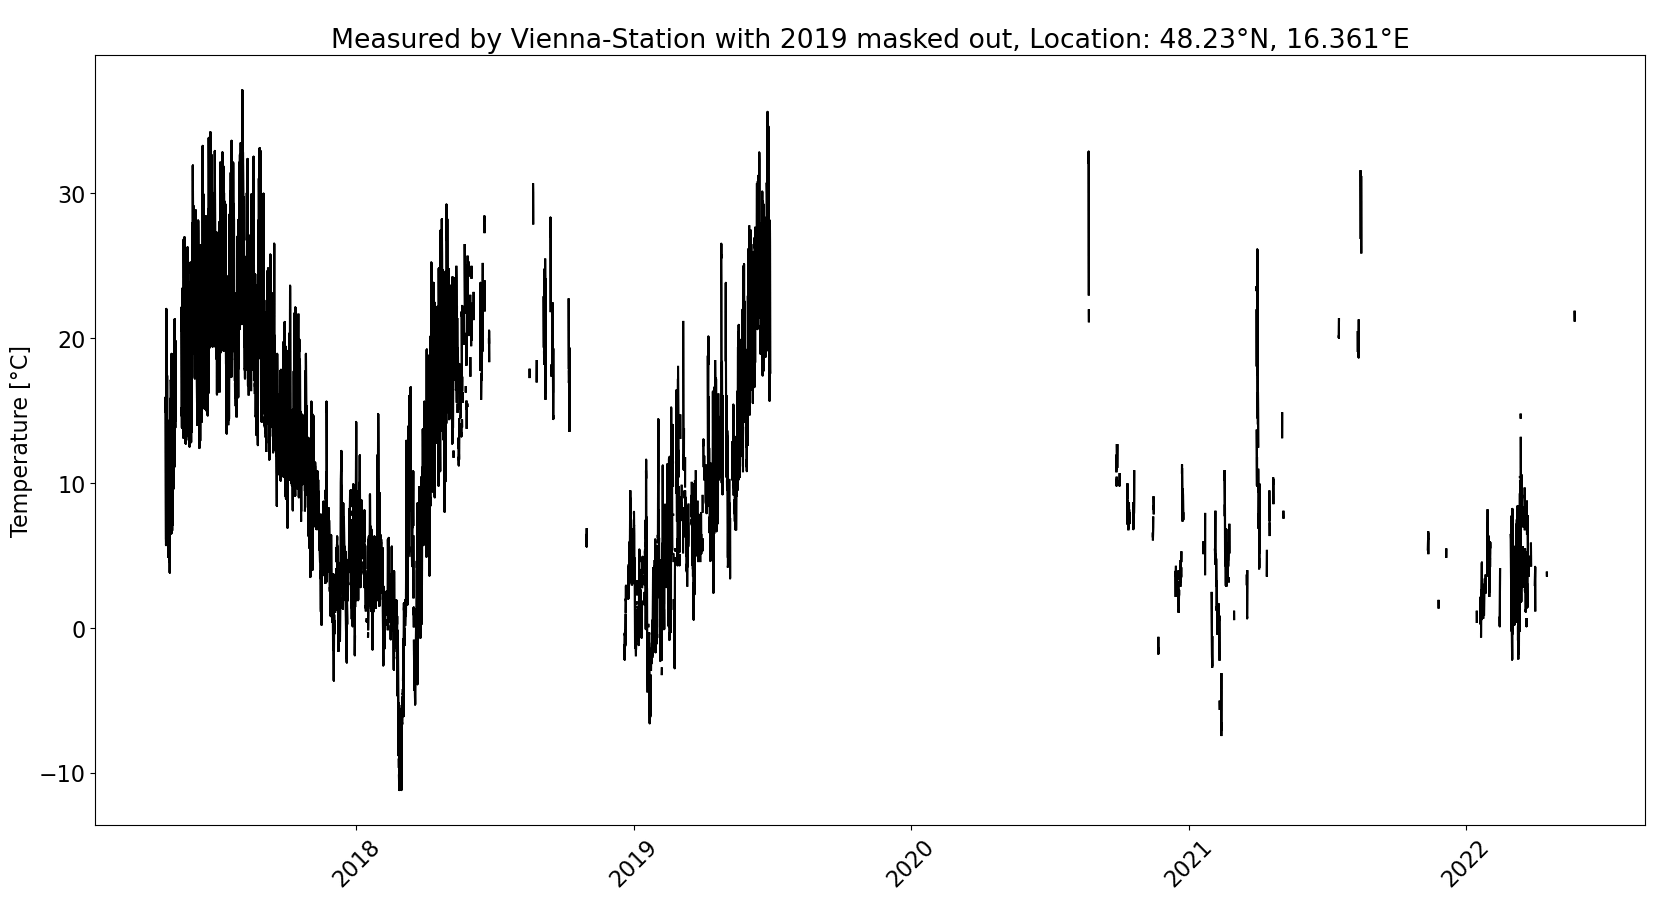
\includegraphics[width=0.8\textwidth]{resources/images/charts/vienna_available_measurements_bw.png}
    \caption{Temperature measurements of a 3D-printed weather station in Vienna, Austria.}
    \label{fig: vienna_measurements}
\end{figure}

% Let's connect aerial data with local measurements

In light of the challenges posed by sparse weather station coverage, novel methodologies are required to address the reconstruction of missing weather data.
Machine learning offers a promising alternative to traditional numerical reconstruction methods, such as kriging, that rely on neighboring station data and are often computationally intensive \cite{chung2019kriging}. Numerical alternatives like Weather Research and Forecasting (WRF) models provide greater accuracy than kriging but are even more computationally demanding \cite{skamarock2008wrf}.
The application of machine learning, in this case, would be to relate coarse-resolution numerical reanalysis data, which in itself can not accurately describe the local characteristics, to the local patterns at the weather station.
This would allow for independent operation without relying on neighboring stations or additional data sources. It can directly utilize the global reanalysis data as input, outperforming numerical methods in terms of computational resource requirements by orders of magnitude \cite{kurth2023MLperformance,bi2023MLperformance,lam2023MLperformance} as the application of the trained machine-learning model.
By leveraging available local data, these techniques, such as Convolutional Neural Networks (CNNs), can be trained to estimate weather conditions at a designated time by assimilating global numerical weather model data.
Despite the inherent blurriness of aerial data provided in grid cells, these models are anticipated to discern and adapt to local weather patterns such that they become capable of transferring knowledge from the meta situation to the local situation.
This paper aims to achieve reconstruction using that approach, which will be further explained in \autoref{sec: design}.

% ERA5 0.25 hourly everywhere

The reanalysis of choice in this endeavor is the ECMWF Reanalysis v5 (ERA5), which covers the globe in grid cells of 0.25° x 0.25°.
The data is available in hourly timesteps from 1940 to the present and contains a wide range of variables, such as temperature, precipitation, wind speed, and many more \cite{era5}.

% Let's go with the temperature

To prove the concept it is likely easiest to start with temperature data, meaning the 2m temperature variable from the ERA5 reanalysis will be used as input to the neural net.

